\documentclass{standalone}
\usepackage{tikz}
\usetikzlibrary{patterns, positioning}


\begin{document}
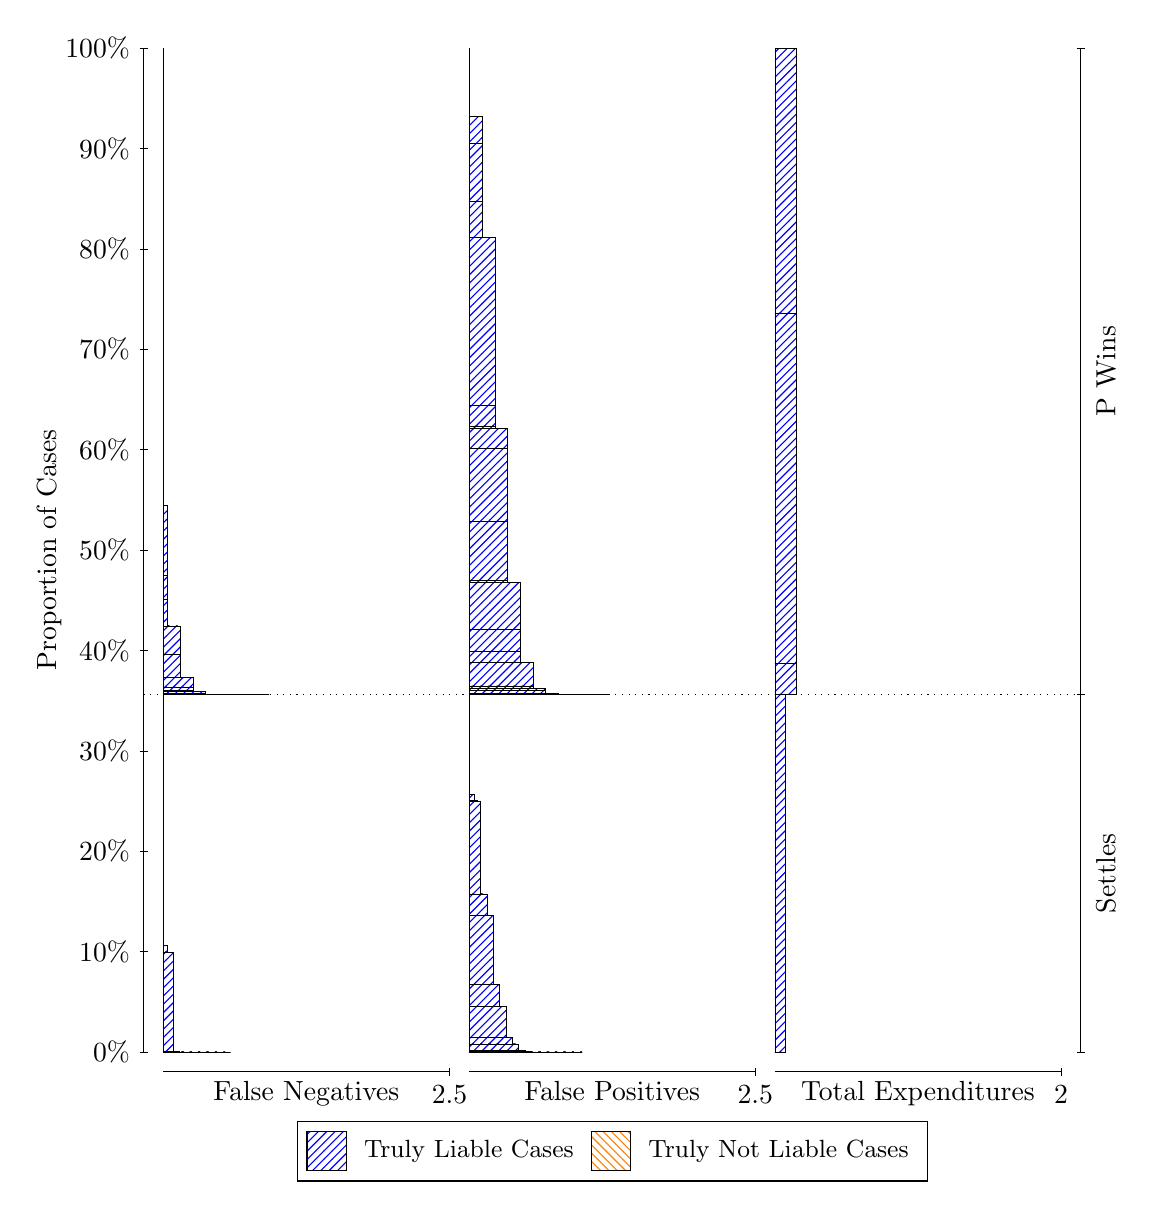
\begin{tikzpicture}
\draw[black, very thin] (1.5,1.75) -- (1.5,14.5);
\node[rotate=90, text=black, anchor=center] at (0.3, 8.125) {Proportion of Cases};
\draw[black, very thin] (1.45,1.75) -- (1.55,1.75);
\node[text=black, anchor=east] at (1.45, 1.75) {0\%};
\draw[black, very thin] (1.45,3.025) -- (1.55,3.025);
\node[text=black, anchor=east] at (1.45, 3.025) {10\%};
\draw[black, very thin] (1.45,4.3) -- (1.55,4.3);
\node[text=black, anchor=east] at (1.45, 4.3) {20\%};
\draw[black, very thin] (1.45,5.575) -- (1.55,5.575);
\node[text=black, anchor=east] at (1.45, 5.575) {30\%};
\draw[black, very thin] (1.45,6.85) -- (1.55,6.85);
\node[text=black, anchor=east] at (1.45, 6.85) {40\%};
\draw[black, very thin] (1.45,8.125) -- (1.55,8.125);
\node[text=black, anchor=east] at (1.45, 8.125) {50\%};
\draw[black, very thin] (1.45,9.4) -- (1.55,9.4);
\node[text=black, anchor=east] at (1.45, 9.4) {60\%};
\draw[black, very thin] (1.45,10.675) -- (1.55,10.675);
\node[text=black, anchor=east] at (1.45, 10.675) {70\%};
\draw[black, very thin] (1.45,11.95) -- (1.55,11.95);
\node[text=black, anchor=east] at (1.45, 11.95) {80\%};
\draw[black, very thin] (1.45,13.225) -- (1.55,13.225);
\node[text=black, anchor=east] at (1.45, 13.225) {90\%};
\draw[black, very thin] (1.45,14.5) -- (1.55,14.5);
\node[text=black, anchor=east] at (1.45, 14.5) {100\%};

\draw[black, very thin] (13.4,1.75) -- (13.4,14.5);
\draw[black, very thin] (13.35,1.75) -- (13.45,1.75);
\node[anchor=west] at (13.35, 1.75) {};
\draw[black, very thin] (13.35,6.2904) -- (13.45,6.2904);
\node[anchor=west] at (13.35, 6.2904) {};
\draw[black, very thin] (13.35,14.5) -- (13.45,14.5);
\node[anchor=west] at (13.35, 14.5) {};

\draw[black, very thin, pattern color=blue, pattern=north east lines] (1.75,1.75) rectangle (2.6038,1.75);
\draw[black, very thin, pattern color=blue, pattern=north east lines] (1.75,1.75) rectangle (2.4424,1.75);
\draw[black, very thin, pattern color=blue, pattern=north east lines] (1.75,1.75) rectangle (2.2809,1.75);
\draw[black, very thin, pattern color=blue, pattern=north east lines] (1.75,1.75) rectangle (2.2405,1.75);
\draw[black, very thin, pattern color=blue, pattern=north east lines] (1.75,1.75) rectangle (2.1194,1.7502);
\draw[black, very thin, pattern color=blue, pattern=north east lines] (1.75,1.7502) rectangle (2.079,1.7502);
\draw[black, very thin, pattern color=blue, pattern=north east lines] (1.75,1.7502) rectangle (1.9579,1.7575);
\draw[black, very thin, pattern color=blue, pattern=north east lines] (1.75,1.7575) rectangle (1.9175,1.7575);
\draw[black, very thin, pattern color=blue, pattern=north east lines] (1.75,1.7575) rectangle (1.8772,3.0211);
\draw[black, very thin, pattern color=blue, pattern=north east lines] (1.75,3.0211) rectangle (1.7964,3.1001);
\draw[black, very thin, pattern color=blue, pattern=north east lines] (1.75,3.1001) rectangle (1.7561,3.1002);
\draw[black, very thin, pattern color=orange, pattern=north west lines] (1.75,3.1002) rectangle (1.75,3.1002);
\draw[black, very thin, pattern color=blue, pattern=north east lines] (1.75,3.1002) rectangle (1.75,6.2904);
\draw[black, very thin, pattern color=blue, pattern=north east lines] (1.75,6.2904) rectangle (3.0943,6.2904);
\draw[black, very thin, pattern color=blue, pattern=north east lines] (1.75,6.2904) rectangle (2.9329,6.2904);
\draw[black, very thin, pattern color=blue, pattern=north east lines] (1.75,6.2904) rectangle (2.7714,6.2904);
\draw[black, very thin, pattern color=blue, pattern=north east lines] (1.75,6.2904) rectangle (2.7714,6.2904);
\draw[black, very thin, pattern color=blue, pattern=north east lines] (1.75,6.2904) rectangle (2.6099,6.2906);
\draw[black, very thin, pattern color=blue, pattern=north east lines] (1.75,6.2906) rectangle (2.6099,6.2906);
\draw[black, very thin, pattern color=blue, pattern=north east lines] (1.75,6.2906) rectangle (2.4484,6.2906);
\draw[black, very thin, pattern color=blue, pattern=north east lines] (1.75,6.2906) rectangle (2.4484,6.2926);
\draw[black, very thin, pattern color=blue, pattern=north east lines] (1.75,6.2926) rectangle (2.4484,6.2938);
\draw[black, very thin, pattern color=blue, pattern=north east lines] (1.75,6.2938) rectangle (2.2869,6.3084);
\draw[black, very thin, pattern color=blue, pattern=north east lines] (1.75,6.3084) rectangle (2.2869,6.326);
\draw[black, very thin, pattern color=blue, pattern=north east lines] (1.75,6.326) rectangle (2.1254,6.3425);
\draw[black, very thin, pattern color=blue, pattern=north east lines] (1.75,6.3425) rectangle (2.1254,6.3875);
\draw[black, very thin, pattern color=blue, pattern=north east lines] (1.75,6.3875) rectangle (2.1254,6.509);
\draw[black, very thin, pattern color=blue, pattern=north east lines] (1.75,6.509) rectangle (1.964,6.7992);
\draw[black, very thin, pattern color=blue, pattern=north east lines] (1.75,6.7992) rectangle (1.964,7.16);
\draw[black, very thin, pattern color=blue, pattern=north east lines] (1.75,7.16) rectangle (1.8025,7.5011);
\draw[black, very thin, pattern color=blue, pattern=north east lines] (1.75,7.5011) rectangle (1.8025,7.7993);
\draw[black, very thin, pattern color=blue, pattern=north east lines] (1.75,7.7993) rectangle (1.8025,8.696);
\draw[black, very thin, pattern color=orange, pattern=north west lines] (1.75,8.696) rectangle (1.75,8.696);
\draw[black, very thin, pattern color=blue, pattern=north east lines] (1.75,8.696) rectangle (1.75,14.5);
\draw[black, very thin, pattern color=orange, pattern=north west lines] (5.6333,1.75) rectangle (7.0685,1.75);
\draw[black, very thin, pattern color=blue, pattern=north east lines] (5.6333,1.75) rectangle (7.0685,1.75);
\draw[black, very thin, pattern color=blue, pattern=north east lines] (5.6333,1.75) rectangle (6.907,1.75);
\draw[black, very thin, pattern color=blue, pattern=north east lines] (5.6333,1.75) rectangle (6.7455,1.75);
\draw[black, very thin, pattern color=orange, pattern=north west lines] (5.6333,1.75) rectangle (6.7052,1.75);
\draw[black, very thin, pattern color=blue, pattern=north east lines] (5.6333,1.75) rectangle (6.7052,1.75);
\draw[black, very thin, pattern color=blue, pattern=north east lines] (5.6333,1.75) rectangle (6.5841,1.7502);
\draw[black, very thin, pattern color=blue, pattern=north east lines] (5.6333,1.7502) rectangle (6.5437,1.7502);
\draw[black, very thin, pattern color=blue, pattern=north east lines] (5.6333,1.7502) rectangle (6.4226,1.7576);
\draw[black, very thin, pattern color=blue, pattern=north east lines] (5.6333,1.7576) rectangle (6.3822,1.7576);
\draw[black, very thin, pattern color=orange, pattern=north west lines] (5.6333,1.7576) rectangle (6.3418,1.7576);
\draw[black, very thin, pattern color=blue, pattern=north east lines] (5.6333,1.7576) rectangle (6.3418,1.7689);
\draw[black, very thin, pattern color=blue, pattern=north east lines] (5.6333,1.7689) rectangle (6.2611,1.8536);
\draw[black, very thin, pattern color=blue, pattern=north east lines] (5.6333,1.8536) rectangle (6.2207,1.8537);
\draw[black, very thin, pattern color=blue, pattern=north east lines] (5.6333,1.8537) rectangle (6.1804,1.9384);
\draw[black, very thin, pattern color=blue, pattern=north east lines] (5.6333,1.9384) rectangle (6.0996,2.3315);
\draw[black, very thin, pattern color=blue, pattern=north east lines] (5.6333,2.3315) rectangle (6.0592,2.332);
\draw[black, very thin, pattern color=blue, pattern=north east lines] (5.6333,2.332) rectangle (6.0189,2.605);
\draw[black, very thin, pattern color=blue, pattern=north east lines] (5.6333,2.605) rectangle (5.9381,3.4841);
\draw[black, very thin, pattern color=blue, pattern=north east lines] (5.6333,3.4841) rectangle (5.8978,3.4847);
\draw[black, very thin, pattern color=blue, pattern=north east lines] (5.6333,3.4847) rectangle (5.8574,3.7565);
\draw[black, very thin, pattern color=blue, pattern=north east lines] (5.6333,3.7565) rectangle (5.7766,4.9402);
\draw[black, very thin, pattern color=blue, pattern=north east lines] (5.6333,4.9402) rectangle (5.7363,4.9403);
\draw[black, very thin, pattern color=blue, pattern=north east lines] (5.6333,4.9403) rectangle (5.6959,5.0193);
\draw[black, very thin, pattern color=blue, pattern=north east lines] (5.6333,5.0193) rectangle (5.6333,6.2904);
\draw[black, very thin, pattern color=orange, pattern=north west lines] (5.6333,6.2904) rectangle (7.4137,6.2904);
\draw[black, very thin, pattern color=blue, pattern=north east lines] (5.6333,6.2904) rectangle (7.4137,6.2904);
\draw[black, very thin, pattern color=orange, pattern=north west lines] (5.6333,6.2904) rectangle (7.2522,6.2904);
\draw[black, very thin, pattern color=blue, pattern=north east lines] (5.6333,6.2904) rectangle (7.2522,6.2904);
\draw[black, very thin, pattern color=orange, pattern=north west lines] (5.6333,6.2904) rectangle (7.0907,6.2904);
\draw[black, very thin, pattern color=blue, pattern=north east lines] (5.6333,6.2904) rectangle (7.0907,6.2904);
\draw[black, very thin, pattern color=blue, pattern=north east lines] (5.6333,6.2904) rectangle (6.9292,6.2906);
\draw[black, very thin, pattern color=blue, pattern=north east lines] (5.6333,6.2906) rectangle (6.9292,6.2907);
\draw[black, very thin, pattern color=orange, pattern=north west lines] (5.6333,6.2907) rectangle (6.9292,6.2907);
\draw[black, very thin, pattern color=blue, pattern=north east lines] (5.6333,6.2907) rectangle (6.9292,6.2911);
\draw[black, very thin, pattern color=blue, pattern=north east lines] (5.6333,6.2911) rectangle (6.7677,6.2938);
\draw[black, very thin, pattern color=orange, pattern=north west lines] (5.6333,6.2938) rectangle (6.7677,6.2938);
\draw[black, very thin, pattern color=blue, pattern=north east lines] (5.6333,6.2938) rectangle (6.7677,6.2975);
\draw[black, very thin, pattern color=blue, pattern=north east lines] (5.6333,6.2975) rectangle (6.7677,6.2993);
\draw[black, very thin, pattern color=blue, pattern=north east lines] (5.6333,6.2993) rectangle (6.6063,6.3399);
\draw[black, very thin, pattern color=orange, pattern=north west lines] (5.6333,6.3399) rectangle (6.6063,6.3399);
\draw[black, very thin, pattern color=blue, pattern=north east lines] (5.6333,6.3399) rectangle (6.6063,6.3658);
\draw[black, very thin, pattern color=blue, pattern=north east lines] (5.6333,6.3658) rectangle (6.4448,6.3996);
\draw[black, very thin, pattern color=orange, pattern=north west lines] (5.6333,6.3996) rectangle (6.4448,6.3996);
\draw[black, very thin, pattern color=blue, pattern=north east lines] (5.6333,6.3996) rectangle (6.4448,6.698);
\draw[black, very thin, pattern color=blue, pattern=north east lines] (5.6333,6.698) rectangle (6.2833,6.8428);
\draw[black, very thin, pattern color=blue, pattern=north east lines] (5.6333,6.8428) rectangle (6.2833,7.1119);
\draw[black, very thin, pattern color=orange, pattern=north west lines] (5.6333,7.1119) rectangle (6.2833,7.1119);
\draw[black, very thin, pattern color=blue, pattern=north east lines] (5.6333,7.1119) rectangle (6.2833,7.714);
\draw[black, very thin, pattern color=blue, pattern=north east lines] (5.6333,7.714) rectangle (6.1218,7.7368);
\draw[black, very thin, pattern color=blue, pattern=north east lines] (5.6333,7.7368) rectangle (6.1218,8.4848);
\draw[black, very thin, pattern color=orange, pattern=north west lines] (5.6333,8.4848) rectangle (6.1218,8.4848);
\draw[black, very thin, pattern color=blue, pattern=north east lines] (5.6333,8.4848) rectangle (6.1218,9.4189);
\draw[black, very thin, pattern color=blue, pattern=north east lines] (5.6333,9.4189) rectangle (6.1218,9.6685);
\draw[black, very thin, pattern color=blue, pattern=north east lines] (5.6333,9.6685) rectangle (5.9603,9.7016);
\draw[black, very thin, pattern color=blue, pattern=north east lines] (5.6333,9.7016) rectangle (5.9603,9.966);
\draw[black, very thin, pattern color=orange, pattern=north west lines] (5.6333,9.966) rectangle (5.9603,9.966);
\draw[black, very thin, pattern color=blue, pattern=north east lines] (5.6333,9.966) rectangle (5.9603,12.094);
\draw[black, very thin, pattern color=blue, pattern=north east lines] (5.6333,12.094) rectangle (5.7989,12.56);
\draw[black, very thin, pattern color=blue, pattern=north east lines] (5.6333,12.56) rectangle (5.7989,13.293);
\draw[black, very thin, pattern color=blue, pattern=north east lines] (5.6333,13.293) rectangle (5.7989,13.63);
\draw[black, very thin, pattern color=blue, pattern=north east lines] (5.6333,13.63) rectangle (5.6374,14.281);
\draw[black, very thin, pattern color=blue, pattern=north east lines] (5.6333,14.281) rectangle (5.6333,14.5);
\draw[black, very thin, pattern color=orange, pattern=north west lines] (9.5167,1.75) rectangle (9.6529,1.75);
\draw[black, very thin, pattern color=blue, pattern=north east lines] (9.5167,1.75) rectangle (9.6529,6.2904);
\draw[black, very thin, pattern color=orange, pattern=north west lines] (9.5167,6.2904) rectangle (9.7892,6.2904);
\draw[black, very thin, pattern color=blue, pattern=north east lines] (9.5167,6.2904) rectangle (9.7892,6.6844);
\draw[black, very thin, pattern color=orange, pattern=north west lines] (9.5167,6.6844) rectangle (9.7892,6.6844);
\draw[black, very thin, pattern color=blue, pattern=north east lines] (9.5167,6.6844) rectangle (9.7892,11.136);
\draw[black, very thin, pattern color=orange, pattern=north west lines] (9.5167,11.136) rectangle (9.7892,11.136);
\draw[black, very thin, pattern color=blue, pattern=north east lines] (9.5167,11.136) rectangle (9.7892,14.5);
\draw[black, dotted] (1.5,6.2904) -- (13.4,6.2904);
\draw[black, very thin] (1.75,1.5) -- (5.3833,1.5);
\node[text=black, anchor=north] at (3.5667, 1.5) {False Negatives};
\draw[black, very thin] (5.3833,1.45) -- (5.3833,1.55);
\node[text=black, anchor=north] at (5.3833, 1.45) {2.5};

\draw[black, very thin] (5.6333,1.5) -- (9.2667,1.5);
\node[text=black, anchor=north] at (7.45, 1.5) {False Positives};
\draw[black, very thin] (9.2667,1.45) -- (9.2667,1.55);
\node[text=black, anchor=north] at (9.2667, 1.45) {2.5};

\draw[black, very thin] (9.5167,1.5) -- (13.15,1.5);
\node[text=black, anchor=north] at (11.333, 1.5) {Total Expenditures};
\draw[black, very thin] (13.15,1.45) -- (13.15,1.55);
\node[text=black, anchor=north] at (13.15, 1.45) {2};

\node[text=black, centered, rotate=90] at (13.72, 4.0202) {Settles};
\node[text=black, centered, rotate=90] at (13.72, 10.395) {P Wins};

\draw (7.449999999999999,1.5) node[draw=none] (baseCoordinate) {};
\begin{scope}[align=center]
        \matrix[scale=0.5, draw=black, below=0.5cm of baseCoordinate, nodes={draw}, column sep=0.1cm]{
            \node[rectangle, draw, minimum width=0.5cm, minimum height=0.5cm, pattern color=blue, pattern=north east lines] {}; &
            \node[draw=none, font=\small, text=black] (B) {Truly Liable Cases}; &
            \node[rectangle, draw, minimum width=0.5cm, minimum height=0.5cm, pattern color=orange, pattern=north west lines] {}; &
            \node[draw=none, font=\small, text=black] (B) {Truly Not Liable Cases}; \\
            };
\end{scope}

\end{tikzpicture}
\end{document}